\section*{Aufgabe 4}

Es seien $M$, $N$, $K$ beliebige Mengen. Beweisen Sie folgende Aussagen:\\

a) $(N \ \backslash \ M) \ \backslash \ K = N \ \backslash \ (M \cup K)$\\

(I) Wir zeigen $\text{\textit{linke Seite}} \Rightarrow \text{\textit{rechte Seite}}$
\begin{align*}
(N \ \backslash \ M) \ \backslash \ K &\Rightarrow x \in ((N \ \backslash M) \ \backslash \ K)\\
&\Rightarrow (x \in N \land x \not \in M) \land x \not \in K\\
&\Rightarrow x \in N \land x \not \in M \land x \not \in K\\
&\Rightarrow x \in N \land (x \not \in M \land x \not \in K)\\
&\Rightarrow x \in N \land x \not \in (M \lor K)\\
&\Rightarrow x \in (N \ \backslash \ (M \cup K))\\
&\Rightarrow (N \ \backslash \ (M \cup K)\\
\end{align*}

(II) Wir zeigen $\text{\textit{rechte Seite}} \Rightarrow \text{\textit{linke Seite}}$
\begin{align*}
N \ \backslash \ (M \cup K) &\Rightarrow x \in (N \ \backslash \ (M \cup K))\\
&\Rightarrow x \in N \land x \not \in (M \lor K)\\
&\Rightarrow x \in N \land (x \not \in M \land x \not \in K)\\
&\Rightarrow x \in N \land x \not \in M \land x \not \in K\\
&\Rightarrow (x \in N \land x \not \in M) \land x \not \in K\\
&\Rightarrow x \in ((N \ \backslash M) \ \backslash \ K)\\
&\Rightarrow (N \ \backslash \ M) \ \backslash \ K
\end{align*}

\begin{FlushRight}
$\Box$
\end{FlushRight}

\newpage

b) $N \ \backslash \ (N \ \backslash \ M) = M \Leftrightarrow M \subseteq N$

\begin{align*}
\overbrace{N \ \backslash \ (N \ \backslash \ M) = M}^{\text{linke Seite}} \Leftrightarrow \overbrace{M \subseteq N}^{\text{rechte Seite}}
\end{align*}

(I) Rechte Seite
\begin{align*}
x \in M \Rightarrow x \in N\\
\lnot(x \in M) \lor (x \in N)\\
(x \not \in M) \lor (x \in N)
\end{align*}

(II) Linke Seite
\begin{align*}
x \in N \land x \not \in (x \in N \land x \not \in M) &= x \in M\\
x \in N \land (x \not \in N \lor x \in M) &= x \in M\\
(x \in N \land x \not \in N) \lor (x \in N \land x \in M) &= x \in M\\
0 \lor (x \in N \land x \in M) &= x \in M\\
x \in N \land x \in M &= x \in M
\end{align*}

(III) Linke Seite $\Leftrightarrow$ Rechte Seite

\begin{figure}[h]
\centering
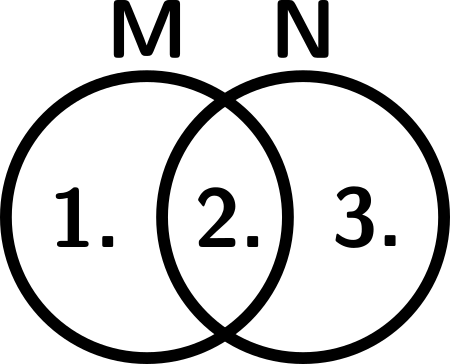
\includegraphics[width=0.2\textwidth]{graphics/proof.png}
\end{figure}

\begin{align*}
1. (\overbrace{0}^{N} \land \overbrace{1}^{M}) = 1 &\Leftrightarrow 0 = 0\\
2. (\overbrace{1}^{N} \land \overbrace{1}^{M}) = 1 &\Leftrightarrow 1 = 1\\
3. (\overbrace{1}^{N} \land \overbrace{1}^{M}) = 0 &\Leftrightarrow 1 = 1
\end{align*}

c) $M \subseteq N \Leftrightarrow M \ \backslash \ N = \emptyset$

\newpage